\documentclass[12pt]{article}
\usepackage{indentfirst}
\usepackage[utf8x]{inputenc}
\usepackage[T1]{fontenc}
\usepackage[english,lithuanian]{babel}
\usepackage{array}
\usepackage{caption}
\usepackage{makecell}
\usepackage[euler]{textgreek}
\usepackage{multirow}
\usepackage{boldline}
\usepackage{floatrow}
\floatsetup[table]{capposition=top}
\usepackage{amsmath, amsthm, amssymb}
\usepackage{graphicx}
\usepackage{setspace}
\usepackage{verbatim}
\usepackage[left=3cm,top=2cm,right=1.5cm,bottom=2cm]{geometry}
\usepackage{floatrow}
\newfloatcommand{capbtabbox}{table}[][\FBwidth]
\usepackage{blindtext}
\onehalfspacing
\usepackage[hidelinks, unicode]{hyperref}
\usepackage{textcomp}

\newcommand{\EE}{\mathbb{E}\,} % Mean
\newcommand{\ee}{{\mathrm e}}  % nice exponent
\newcommand{\dd}{{\mathrm d}}
\newcommand{\RR}{\mathbb{R}}

\begin{document}
\selectlanguage{lithuanian}

\begin{titlepage}
\vskip 20pt
\begin{center}

\includegraphics[scale=0.5]{MIF}
\end{center}

%%%%%%%%%%%%%%%%%%%%%%%
% TITULINIS PUSLAPIS
%%%%%%%%%%%%%%%%%%%%%%%

\vskip 20pt
\centerline{\bf \large \textbf{VILNIAUS UNIVERSITETAS}}
\bigskip
\centerline{\large \textbf{MATEMATIKOS IR INFORMATIKOS FAKULTETAS}}
\bigskip
\centerline{\large \textbf{BIOINFORMATIKOS BAKALAURO STUDIJŲ PROGRAMA}}

\vskip 90pt
\begin{center}
    {\bf \LARGE Pavadinimas lietuviškai}
\end{center}
\begin{center}
    {\bf \Large Pavadinimas angliškai}
\end{center}
\vskip 20pt
\centerline{\bf \large \textbf{Kursinis projektas}}
\bigskip
\vskip 40pt

\hskip 140pt {\large Autorė: Danielė Stasiūnaitė}

\hskip 140pt{\large VU el. p.: daniele.stasiunaite@gmc.vu.lt}
\bigskip
\vskip 20pt

\hskip 140pt {\large Darbo vadovė: J. m. d. Kotryna Kvederavičiūtė}
\vskip 60pt
\vskip 40pt
\centerline{\large \textbf{Vilnius}}
\centerline{\large \textbf{2022}}
\newpage
\end{titlepage}

\selectlanguage{lithuanian}

%%%%%%%%%%%%%%%%%%%%%
% TURINIO PUSLAPIS
%%%%%%%%%%%%%%%%%%%%%

\tableofcontents
\newpage

%%%%%%%%%%%%%%%%%%%%%%%%%%%%%%%%%%%%
% LIETUVIŠKOS SANTRAUKOS PUSLAPIS
%%%%%%%%%%%%%%%%%%%%%%%%%%%%%%%%%%%%

\section*{Santrauka}
\newpage

%%%%%%%%%%%%%%%%%%%%%%%%%%%%%%%%%%
% ANGLIŠKOS SANTRAUKOS PUSLAPIS
%%%%%%%%%%%%%%%%%%%%%%%%%%%%%%%%%%

\section*{Summary}
\newpage

%%%%%%%%%%%%%%%%%%%
% ĮVADO PUSLAPIS
%%%%%%%%%%%%%%%%%%%

\section{Įvadas}
\subsection*{Darbo temos aktualumas}
\subsection*{Darbo tikslas}
\subsection*{Uždaviniai}

\newpage

%%%%%%%%%%%%%%%%%%%%%%%%%%%%%%%%%%%%%%
% SYNTENY BLOKŲ IDENTIFIKAVIMO METODAI
%%%%%%%%%%%%%%%%%%%%%%%%%%%%%%%%%%%%%%

\section{\emph{Synteny} blokai ir jų identifikavimo metodai}
\subsection{\emph{Synteny} bloko apibūdinimas}

\textbf{\emph{Synteny} blokas} - tarp skirtingų genomų identifikuojami
chromosomų regionai, kuriems būdingi bendri homologiniai genai, 
išsidėstę nebūtinai vienoda tvarka. \emph{Synteny} blokai neretai gali būti
vadinami kolineariais blokais. Pastarieji blokai nuo \emph{synteny} blokų
skiriasi tik tuo, kad kolineariesiems blokams būdingas identiškas genų
išsidėstymas. Žemiau pateikiamame pirmame paveiksle (1 pav.) vaizduojami
\emph{synteny} blokų tipai:

\begin{figure}[htb]
    \begin{center}
        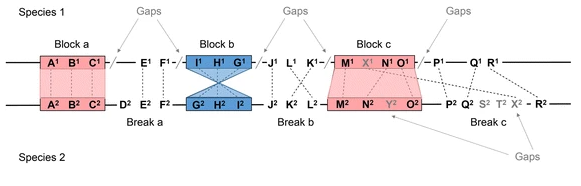
\includegraphics[width=0.7\linewidth]{../Figures/Synteny_blocks.png}
        \vspace{-2\baselineskip}
        \caption*{\small\textbf{1 pav. \emph{Synteny} blokų tipai.
        \href{https://bmcbioinformatics.biomedcentral.com/articles/\
        10.1186/s12859-018-2026-4}{\emph{Inferring synteny between genome assemblies:
        a systematic evaluation}}}}
        \label{fig:birds}
    \end{center}
\end{figure}

Paveiksle vaizduojamuose blokuose yra po tris ortologinius genus (inkarus):
\begin{enumerate}
    \item \textbf{A blokas:} \emph{synteny} blokas tarp vienoda tvarka
    išsidėsčiusių ortologinių genų;
    \item \textbf{B blokas:} \emph{synteny} blokas tarp priešinga tvarka
    išsidėsčiusių ortologinių genų;
    \item \textbf{C blokas:} \emph{synteny} blokas tarp ortologinių genų,
    kuriuos skiria neortologiniai genai.
\end{enumerate}

\subsection{Identifikavimo metodai}
Internete yra viešai prieinamų duomenų bazių (\emph{Ensembl, Synteny portal, 
Genomicus, ECRbase} (DNR lygmenyje)), kuriose yra saugomi tarp
skirtingų organizmų genomų identifikuotų \emph{synteny} blokų duomenys bei
jų aprašymai, tačiau šiose duomenų bazėse yra patalpinta ne visų įmanomų genomų
palyginimo metu identifikuotų \emph{synteny} blokų informacija. Dėl to, yra
sukurta daug įvairių programinių įrankių, leidžiančių atlikti pastarųjų blokų
paiešką savarankiškai. Šiuos įrankius galima pasirinkti pagal tai, koks yra
organizmų giminingumas, koks genomo tyrimas yra atliekamas ir ką norima
sužinoti.

Antrame paveiksle (2 pav.) pateiktoje schemoje vaizduojami metodai išskaidyti
pagal lyginamų genomų giminingumą:

\begin{figure}[htb]
    \begin{center}
        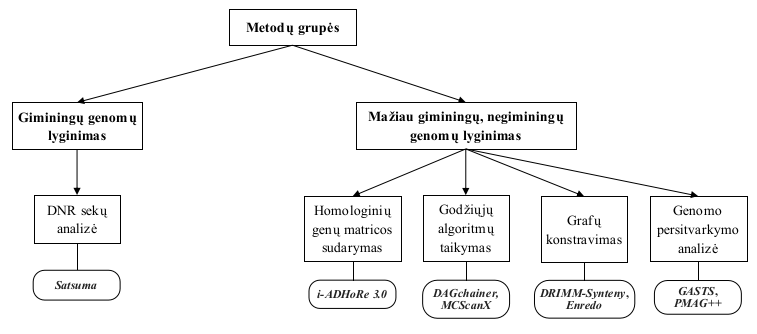
\includegraphics[width=0.9\linewidth]{../Figures/Methods_tools.png}
        \vspace{-2\baselineskip}
        \caption*{\small\textbf{2 pav. \emph{Synteny} blokų identifikavimo
        metodai bei populiariausių įrankių pavyzdžiai}}
        \label{fig:birds}
    \end{center}
\end{figure}

\newpage

\subsubsection{Giminingų organizmų genomų lyginimas}
Lyginant genomus, priklausančius itin giminingiems organizmams, \emph{synteny}
blokai gali būti identifikuojami taikant įrankius, paremtus DNR sekų
išlyginimais, nes genomų sekų atitikimo laipsnis yra didelis (didelė dalis
nukleotidų sutampa).

Konservatyvių chromosomų regionų nustatymui naudojami DNR sekų išlyginimu
paremti metodai yra intuityvūs, tačiau reikalaujantys didelių kompiuterio
resursų (jeigu tarpusavyje lyginami eukariotinių organizmų genomai).
Nepaisant to, yra sukurta įrankių, kurie ne tik sprendžia kompiuterio resursų
naudojimo problemą, bet ir pateikia patikimus rezultatus.

Populiariausias DNR sekų išlyginimu paremtą metodą taikantis įrankis yra
\emph{Satsuma}\cite{SATSUMA}. Šis įrankis realizuoja \textbf{kryžminės
koreliacijos metodą}, paremtą sekų išlyginimais. Originaliai šis metodas yra
taikomas, tiriant vienodus garsus bei tarp jų atsirandantį atgarsį, tačiau jis
yra pritaikomas ir analizuojant skirtingų organizmų genomus bei ieškant
homologinių DNR sekų (fragmentų), kurios evoliucijos eigoje pakito. Žemiau
pateikiamas šio metodo aprašymas:
\begin{enumerate}
    \item Užklausos (angl. \emph{query}) ir taikinio (angl. \emph{target})
    sekos suskaidomos į 4096 bazių porų ilgio fragmentus (langus).

    \item Lyginant užklausos ir taikinio sekų langus, kiekvieno lango
    nukleotidai paverčiami keturiais signalais (nukleotidams A, T, C, G).

    \item Kiekvienai signalo porai pritaikoma kryžminė koreliacija ir
    suskaičiuojamas kiekvieno signalo panašumas (jei nukleotidai sutampa,
    sutapimas lygus 1, jei nesutampa - 0).
    
    \item Sutampančių ir nesutampančių nukleotidų vertės susumuojamos -
    gaunama nukleotidų panašumo vertė. Kuo vertė didesnė, tuo didesnė
    dalis nukleotidų tarp dviejų langų sutampa.

    \item \colorbox{yellow}{PRATĘSTI...}

    % While random base matches are expected and constitute background noise,
    % a higher-than-average number of bases that match due to homology produce
    % a signal that rises above the noise. 
\end{enumerate}

\subsubsection{Mažai giminingų arba negiminingų organizmų genomų lyginimas}
Jeigu tiriami tos pačios biologinės klasifikacijos taksonominio rango, klasės,
organizmai, kurie kilę iš bendro protėvio ir turi panašią sandarą, metodai,
kurie remiasi DNR sekų išlyginimu, negali būti taikomi, nes lyginamų organizmų
DNR sekos yra pakitusios (evoliucijos eigoje įvyko daugiau įvairių mutacijų),
todėl \emph{synteny} blokų paieška turi būti atliekama aminorūgščių lygyje,
nes, nepaisant evoliucijos eigoje vykstančių DNR sekų pokyčių, viena
aminorūgštis gali būti koduojama keliais skirtingais kodonais. Dėl šios
priežasties metodo taikymas tinka evoliucijos eigoje mutavusių mažai giminingų
organizmų genomų sekų lyginimui ir homologinių regionų paieškai.

Norint palyginti skirtingoms taksonominėms klasėms priklausančių organizmų
genomus taikomi metodai, analizuojantys baltymus koduojančias aminorūgštis,
bei metodai, konstruojantys profilius, grafus ir naudojantys įvairius
statistinius modelius.

Taikant šiuos metodus yra svarbu, kad analizuojamų organizmų
genomai būtų kuo kokybiškesni. Jeigu genome trūksta sekų, gali nebūti
tam tikrų genų anotacijų, todėl ortologinių sąsajų taip pat nebūtų galima
tyrinėti - kai kurie \emph{synteny} blokai nebūtų identifikuoti.

\subsubsection*{Homologinių genų matricos sudarymo metodas}

Taikant šį metodą, \emph{synteny} blokai identifikuojami, naudojant kaimyninių
genų porų klasterizavimą. Genomų genų atitikimai arba neatitikimai fiksuojami
matricoje. Jeigu genai homologiniai, matricoje įrašomas '1', jei nehomologiniai
- įrašomas '0'. Remiantis šiuo metodu \emph{synteny} blokai nustatomi, ieškant,
kurioje matricos diagonalės vietoje yra didžiausia vienetų sankaupa.

\textbf{Metodo privalumas:} taikant šį metodą nustatytiems \emph{synteny}
blokams galima paprastai pritaikyti statistinę validaciją ir aptikti
\emph{false positive} reikšmes.

\textbf{Metodo trūkumai:} taikant šį metodą yra svarbu tiksliai žinoti, į kokį
biologinį klausimą norima atsakyti, nes nuo to priklauso, koks paieškai
reikalingas parametras arba jų konfigūracijos bus pasirinktos, jog būtų gauti
optimalūs rezultatai. Pavyzdžiui, tarpo tarp dviejų genų dydis, kuris gali
egzistuoti identifikuotame \emph{synteny} bloke. Kuo šio parametro vertė
mažesnė, tuo daugiau nedidelių ir sunkiai analizuojamų \emph{synteny} blokų
bus identifikuota, tačiau, jei tarpo ilgio parametro reikšmė didelė,
identifikuotas blokas bus didelis - analizės atlikimas taps paprastesniu. Kita
vertus, tokiame bloke gali atsirasti tokių sekų fragmentų, kurie iš tiesų
neturėtų priklausyti blokui (daugiau \emph{false positive} reikšmių), nes nėra
aptinkami kitame genome. Taip pat taikant šį metodą keblu atsižvelgti į genų
pasikartojimus bei identifikuoti inversijas ir nepersidengiančius
\emph{synteny} blokus.

Šis metodas taikomas įrankyje \emph{i-ADHoRe 3.0}\cite{IADHORE}. Jis leidžia
analizuoti didelį kiekį genomų, atliekant paralelinius skaičiavimus. Šiame
įrankyje į homologinių genų matricą įtraukiami tie genų klasteriai,
kuriuos sudaro bent trys homologinių genų poros ir kuriems atlikus statistinę
validaciją, gaunami patikimi klasterių \emph{p} įverčiai. Jeigu nustatyti keli
klasteriai, atliekama \emph{Bonferroni} arba \emph{FDR} korekcija.

% A syntenic block can be defined as a region of the genome spanning a number of
% genes that are orthologous and co-arranged compared to another genome [154].
% Two regions of a genome with a number of homologous genes co-arranged with
% each other can also be defined as a syntenic block. Here, we focus on this
% second definition because pairs of homologous genes between these pairs of
% regions correspond to duplicated genes.

\subsubsection*{Godžiųjų algoritmų taikymo metodas}
Šis metodas konstruoja kolinearių genų porų grandines, atlikdamas daug daugiau
skaičiavimų nei aprašytas homologinių genų matricos sudarymo metodas.
Įrankiuose, kurie remiasi šiuo metodu, yra naudojami \emph{BLASTP} rezultatai.
Remiantis jais galima taikyti dinaminį programavimą ir sukonstruoti kolinearių
genų porų grandines, turinčias maksimalias grandinės vertes (angl.
\emph{chainscore}). Taikant šį metodą \emph{synteny} blokus sudaro kolineariose
pozicijose esančių unikalių homologinių sekų (\emph{synteny} inkarų) genai bei
tarp jų išsidėstę nehomologiniai genai, kurie evoliucijos eigoje buvo paveikti
mutacijų.
% one level is bi-directionarily unique homologous sequences between the two 
% genomes (syntenic anchors)

\textbf{Metodo privalumai:} Taikant šį metodą galima lyginti daug skirtingų
genomų ir analizuoti genų pokyčius chromosomose. Taip pat genomų kolinearių
genų paieškos algoritmai veikia itin sparčiai ir pateikia išsamius rezultatus.

\textbf{Metodo trūkumas:} Taikant metodą reikia iš anksto žinoti, ko reikia
ieškoti, bei, kokios yra tiriamų genomų bei \emph{synteny} blokų
charakteristikos.

Šis metodas realizuotas \emph{MCScanX}\cite{MCSCANX} įrankyje. Jame
\emph{synteny} blokai identifikuojami, atlikus \emph{BLASTP} genomų palyginimą,
suradus kolinearius blokus ir juos surikiavus pagal jų genomines pozicijas.
Taikant dinaminį programavimą yra surandamos didžiausią vertę sudarančios
kolinearių genų porų grandinės. Nepersidengiančios grandinės, turinčios bent
penkias kolinearių genų poras, yra išsaugomos - kitų įrankio algoritmo etapų
metu šioms grandinėms priskiriama genų klasė ir atliekamos įvairios analizės.

% % Syntenic anchors (Mural et al., 2002) are sequences in two genomes that
% % show significant sequence similarity and are bi-directionally unique
% % matches (i.e. they are found in only one location in each genome).

\subsubsection*{Grafų konstravimo metodas}
Kai yra žinomos baltymus koduojančių genų pozicijos ir sekų išlyginimo
tikimybė, galima konstruoti grafus, surenkančius visas įmanomas homologinių genų
poras tarp lyginamų genomų.

Iš pradžių yra atliekamas lokalus genomų išlyginimas, po kurio gauti
išlyginimai naudojami grafo konstravimui bei genomų vidinių struktūrų paieškai.
Priklausomai nuo to, kokį grafą bus pasirinkta sukonstruoti, gali būti gauti
labai skirtingi identifikuotų \emph{synteny} blokų rezultatai. Taikant šį
metodą galima konstruoti keturis skirtingus grafus: išlyginimų,
\emph{de-Bruijn}, \emph{Enredo}, \emph{Cactus}. Skirtingų grafų taikymo
privalumai/trūkumai:

\begin{itemize}
    \item \textbf{Išlyginimų grafas:} regionai, kurie pasikartoja keliose
    chromosomos vietose, yra lengviau pastebimi, tačiau šis grafas neatsižvelgia
    į galimą chromosomų inversiją.
    \item \textbf{\emph{De-Bruijn} grafas:} dėl trumpų ciklų susidarymo galima
    nepastebėti lokalaus kolinearumo. Be to, grafas negali padėti nustatyti
    galimos chromosomų inversijos.
    \item \textbf{\emph{Enredo} grafas:} padeda aptikti nepersidengiančius
    \emph{synteny} blokus ir analizuoti nepersidengiančias inversijas.
    \item \textbf{\emph{Cactus} grafas:} padeda aptikti trumpus ciklus.
\end{itemize}

Taikant skirtingus grafų tipus tiriamos vidinės genomo struktūros, jog būtų
identifikuoti \emph{synteny} blokai. Šiomis struktūromis gali būti: iš eilės
einantys ir tarp dviejų genomų sutampantys genų sekų blokai, tarp kurių nėra
tarpų ir kuriems būdinga vienoda kryptis abiejuose genomuose; mikroblokai -
blokai tarp kurių gali būti tarpų; trumpi ciklai, kurie įrodo, kad genomas
pakito, vykstant persitvarkymo procesams.

Grafų konstravimo metodas realizuotas įrankyje
\emph{DRIMM-Synteny}\cite{DRIMM-SYNTENY}.
\colorbox{yellow}{PAPILDYTI APRAŠYMU...}


% Reciprokinis - A reciprocal action or arrangement involves two people or
% groups of people who behave in the same way or agree to helpl each other and
% give each other advantages.


\newpage

\section*{1. Čia aprašyti, koks rezultatas gautas, pasinaudojus
Cinteny įrankiu: pateikti diagramas ir vaizdus}

\section*{2. Aprašyti, kad buvo analizuota, kiek persidengiančių synteny blokų
yra su pikais, tačiau gautas mažas persidengimo procentas}


\newpage

\bibliographystyle{plain}
\begin{thebibliography}{99}

\bibitem{SATSUMA} Grabherr, M. G., Russell, P., Meyer, M., Mauceli,
E., Alföldi, J., Di Palma, F., \& Lindblad-Toh, K. (2010). Genome-wide
synteny through highly sensitive sequence alignment: Satsuma.
Bioinformatics, 26(9), 1145-51.

\bibitem{IADHORE} Proost, S.; Fostier, J.; De Witte, D.; Dhoedt, B.;
Demeester, P.; Van de Peer, Y.; Vandepoele, K. i-ADHoRe 3.0—Fast and sensitive
detection of genomic homology in extremely large data sets. Nucleic Acids Res.
2012, 40, e11.

\bibitem{MCSCANX} Wang Y, Tang H, Debarry JD, Tan X, Li J, Wang X, Lee TH,
Jin H, Marler B, Guo H, Kissinger JC, Paterson AH. MCScanX: a toolkit for
detection and evolutionary analysis of gene synteny and collinearity. Nucleic
Acids Res. 2012 Apr;40(7):e49. doi: 10.1093/nar/gkr1293. Epub 2012 Jan 4.
PMID: 22217600; PMCID: PMC3326336.

\bibitem{DRIMM-SYNTENY} Pham, S.K.; Pevzner, P.A. DRIMM-Synteny: Decomposing
genomes into evolutionary conserved segments. Bioinformatics 2010, 26,
2509–2516.

\bibitem{SYNCHRO} Drillon G, Carbone A, Fischer G (2014) SynChro: A Fast and
Easy Tool to Reconstruct and Visualize Synteny Blocks along Eukaryotic
Chromosomes. PLoS ONE 9(3): e92621. https://doi.org/10.1371/journal.pone.0092621

\bibitem{ARTICLE1} Liu, D., Hunt, M. \& Tsai, I.J. Inferring synteny between
genome assemblies: a systematic evaluation. BMC Bioinformatics 19, 26 (2018).
https://doi.org/10.1186/s12859-018-2026-4

\bibitem{ARTICLE2} Lallemand, T.; Leduc, M.; Landès, C.; Rizzon, C.; Lerat, E.
An Overview of Duplicated Gene Detection Methods: Why the Duplication Mechanism
Has to Be Accounted for in Their Choice. Genes 2020, 11, 1046.
https://doi.org/10.3390/genes11091046

\end{thebibliography}
\end{document}